\documentclass[12pt]{article}
\usepackage[margin=1in]{geometry}
\usepackage{times}
\usepackage{graphicx}
\usepackage{float}
\usepackage{caption}
\usepackage{subcaption}
\usepackage{lineno}
\usepackage{amsmath}
%\usepackage{natbib,hyperref}
\linenumbers

\newcommand*{\met}{\ensuremath{E_\text{T}^\text{miss}}}

\author{Danika MacDonell}
\title{Search for Dark Matter Produced in Association with a Hypothetical Dark Higgs Boson Decaying to $W^+W^-$ in the $q\bar{q}\ell\nu$ Final State Using $pp$ Collisions Recorded with the ATLAS Detector}
\begin{document}
\maketitle

\section{Introduction}

The proposed thesis is a search for dark matter using high energy proton-proton ($pp$) collision data recorded with the ATLAS detector at the Large Hadron Collider (LHC). The search targets a final state signature of dark matter production in association with the emission of a hypothetical higgs boson $s$ in the dark sector, which subsequently decays to a pair of W bosons. The search is motivated by and optimized with a ``dark higgs model" \cite{dark_higgs} shown in figure \ref{fig:signal_model}, in which the $s$ is emitted from a hypothetical $Z'$ gauge boson in the dark sector, which itself mediates the production of dark matter particles from the high energy $pp$ collisions.

Any dark matter that may be produced in the $pp$ collisions is expected not to interact to any measurable extent with the `normal' matter constituting the detector. As such, it is assumed that the momentum carried by the dark matter would escape the detector undetected. However, the law of momentum conservation requires that the momenta of all particles produced by a $pp$ collision in the plane transverse to the beam line sum to zero. This fundamental requirement implies that dark matter produced at the LHC will exhibit a signature of high missing transverse momentum in the final state. The magnitude of this two dimensional missing transverse momentum vector is typically denoted ``\met". 

The aim of the proposed thesis work is to apply selections, including a requirement of high \met, to data from the ATLAS detector to optimize the sensitivity of the data to the dark higgs signal model. The data will subsequently be compared with standard model (SM) background and signal processes simulated with Monte Carlo (MC) to search for an above-background excess in the data consistent with the signal model. 

The search is split into two separate analyses:

\begin{enumerate}

\item \textbf{The hadronic decay channel:} In this channel, each of the two W bosons in the final state decay to quarks, which subsequently hadronize in the detector and are measured as jets in the ATLAS calorimeter.

\begin{equation}
\nonumber
WW \rightarrow q\bar{q}+q\bar{q}
\end{equation}

Given that the branching fraction for hadronic W decay is 0.68 \cite{PDG}, the fully hadronic WW decay occurs with a branching fraction of 0.46 ($=0.68^2$). In addition to its substantial branching fraction, this channel has the advantage of being able to fully reconstruct the momenta of both W bosons, and as such the $s$ mass. The drawback is that there are standard model processes with large production cross section which also produce a final state of multiple jets in the detector, a subset of which pass the other signal selection criteria and represent a sizeable background in the analysis. 

\item \textbf{The semileptonic decay channel:} One W boson decays to quarks in this channel, and the other decays to a lepton and a neutrino, where the lepton is either an electron or a muon. 

\begin{equation}
\nonumber
WW \rightarrow q\bar{q}+\ell\nu
\end{equation}

Despite its lower branching fraction of 0.29 \cite{PDG} compared with the fully hadronic decay channel, the semileptonic channel has the advantage that the requirement of having one lepton in the final state reduces the background from standard model processes. However, this comes at the cost of additional \met from the neutrino production, which both inhibits reconstruction of the leptonically-decaying W boson and cannot easily be distinguished from the \met associated with dark matter production in the signal model. 

\end{enumerate}

There is an ongoing analysis searching for the dark higgs signal in the hadronic decay channel, and the proposed thesis will focus on the semileptonic decay channel. 

The WW decay can also proceed via a fully leptonic channel, in which both W bosons decay to a lepton and a neutrino. This channel would give a clean signature of two leptons and no jets, but is currently not considered as a viable search channel due to its relatively low branching fraction of 0.046 \cite{PDG}.

Once the analysis is fully developed in the semileptonic decay channel, this channel will be statistically combined with the hadronic search channel. In the event that the combined search does not show an above-background excess, the analysis will place exclusion limits - to within some level of confidence, typically 95\% - on the range of $Z'$ and $s$ masses in the dark higgs model to which the combined search is sensitive.

\section{Motivation}

The proposed thesis work would contribute to the extensive ongoing dark matter search program at the LHC. The LHC search program is motivated by compelling evidence from observational astronomy for the existence of dark matter constituting 85\% \cite{planck} of all matter in the universe. Despite clear evidence from observational astronomy for its gravitational interactions with normal matter, dark matter has yet to be detected through the weak, strong or electromagnetic interactions. As such, its composition and non-gravitational interactions - if any - remain largely a mystery. The current most widely accepted and theoretically motivated dark matter candidates take the form of fundamental particles, yet there is no particle in the standard model of particle physics that could represent a viable dark matter candidate \cite{feng}. Dark matter is therefore widely assumed to be a ``beyond-standard-model" (BSM) particle. 

\subsection{Dark Matter Search Methods}
There are three complementary approaches used to search for particle dark matter: direct and indirect detection, and collider searches. Direct detection searches \cite{Schumann_2019, 2015gya} aim to directly detect evidence of a recoil induced by elastic scattering between a dark matter particle in the galactic halo passing through the detector and a target particle in the detector. Indirect searches \cite{CIRELLI_2012, conrad} use observational data to search for evidence of products produced by dark matter annihilation or decay in particular regions of the observable universe expected to have a high dark matter density. Collider searches \cite{DM_colliders}, of which the proposed thesis work is an example, study the decay products from high-energy collisions of subatomic particles to search for an above-background excess of events that could be consistent with dark matter having been produced in some of the collisions.

\subsection{Models of Dark Matter Production at Colliders}
Models of dark matter production in colliders can range in complexity from an effective field theory (EFT), where the dark matter production mechanism is completely unspecified, to a complete model such as supersymmetry \cite{susy_dm}, which predicts viable dark matter candidates as part of a hypothesized extension to the standard model designed to address a range of phenomena unexplained by the standard model. 

%The EFT approach treats the production of dark matter from colliding partons as a contact interaction, with the production rate determined by a single parameter \cite{DM_colliders}. As long as a measurable standard model particle is also produced in the interaction (eg. a gluon radiating from one of the colliding quarks, see figure \ref{fig:eft_simplified_model}), the EFT framework can be applied to any mono-X signature at the LHC, where a SM particle X is measured along with missing transverse momentum in the detector. This makes the framework generally usable in terms of motivating and providing a theoretical framework to interpret a range of generic search channels that can be readily selected for in LHC collision data. However, the EFT framework relies on the assumption that the the mediator(s) of the interaction is (are) much more massive than the scale of momentum transfer in the interaction \cite{DM_colliders, beyond_eft}. If this assumption is inaccurate, the EFT framework becomes invalid, and a more complete model is needed to specify additional details of the process leading to dark matter pair production. 

\begin{figure}[H]
	\centering
	\begin{minipage}[b]{0.45\textwidth}
	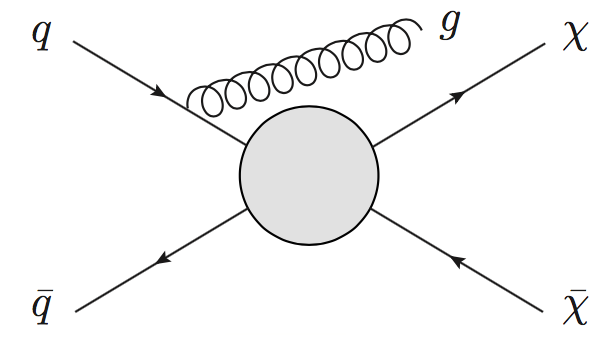
\includegraphics[width=0.9\textwidth]{figures/EFT_Signature.png}
	\end{minipage}
	\begin{minipage}[b]{0.45\textwidth}
	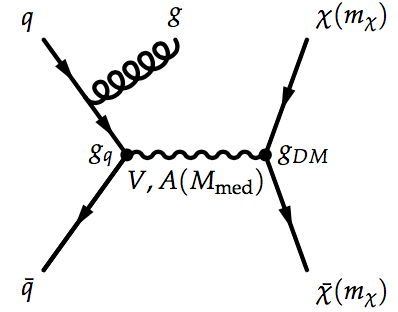
\includegraphics[width=0.8\textwidth]{figures/simplified_model.png}
	\end{minipage}
	\caption[]{Left: Mono-jet process in the EFT framework (source: \cite{beyond_eft}). Right: Mono-jet process in a simplified model framework, where the pair production of dark matter occurs via a new vector or axial-vector ($V$, $A$) mediator of mass $M_\text{med}$, which couples to quarks and dark matter with coupling constants g$_q$ and g$_\text{DM}$, respectively (source: \cite{dm_forum})}
	\label{fig:eft_simplified_model}
\end{figure}

In principle, complete theories of physics beyond the standard model, such as the minimal supersymmetric standard model (MSSM) \cite{mssm} can offer theoretically motivated and experimentally accessible models which specify the details of candidate processes by which the colliding partons may annihilate to produce dark matter. However, these theories tend to be quite complex, with many free parameters - over 100 in the case of MSSM \cite{DM_colliders} - most of which need to be fixed to generate a reasonably testable model. Relying on complete theories alone to guide experimental signatures may run the risk of missing important parameter space of new physics for which a complete theory has not yet been developed. 

Simplified models, widely used in recent and ongoing dark matter searches at the LHC, are designed to bridge the gap between EFT and complete theories. They provide a `first-order' description of theoretically motivated new physics scenarios that could be accessible at collider energies. They provide guidance for experimental searches without fully specifying the details of any additional new physics at energies above the collider scale that would be needed for a complete theory \cite{DM_colliders}. In terms of dark matter production at the LHC, one or more new mediators associated with new physics scenarios may be considered which allow for mixing between standard model particles and dark matter. The process by which the mixing occurs is represented with a tree-level diagram whose experimental signature would be accessible at LHC energies, such as the diagram shown in figure \ref{fig:eft_simplified_model} which represents a dark matter benchmark model featured in the 2015 report of the ATLAS/CMS Dark Matter Forum \cite{dm_forum}.

\subsection{Dark Higgs Model}

The proposed search is motivated by and interpreted with a simplified model described in \cite{dark_higgs} where dark matter is pair produced from a Z boson in the dark sector - known as the $Z'$ boson - in association with the emission of an additional dark sector higgs boson $s$. Figure \ref{fig:signal_model} shows one of the leading order Feynman diagrams representing this simplified model. The dark sector higgs boson subsequently decays to a pair of massive standard model particles through a small mixing with the SM higgs boson. 

\begin{figure}[H]
	\centering
	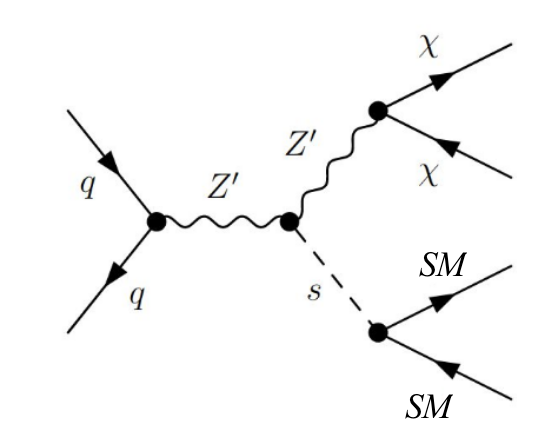
\includegraphics[width=0.4\textwidth]{figures/Signal_generic.png}
	\caption[]{Dark higgs model}
	\label{fig:signal_model}
\end{figure}

The generic hypothesis of `dark sector' mediators which exhibit a small mixing with SM particles is motivated in part by the theoretical need for creation and annihilation mechanisms between DM and SM particles in the well-motivated and popular `thermal freeze-out' hypothesis \cite{particle_dm}. In the thermal freeze-out hypothesis, DM and SM particles interacted at a sufficient rate in the high temperature and matter density of the early universe to remain in thermal equilibrium. Once the DM-SM interaction rate dropped below the expansion rate of the universe, the DM rapidly ``froze out" of thermal equilibrium with the SM particles, at which point the relic abundance of DM was fixed to the value observed in the present-day universe.

The dark higgs boson in particular is motivated by the need to generate the masses of dark matter and any other particles residing in the dark sector \cite{dark_higgs}. If dark sector particle masses are generated via a `dark sector higgs mechanism', this would naturally imply the existence of a dark higgs boson. 

The model presented in \cite{dark_higgs} considers a scenario in which there is another dark sector mediator - taken to be the $Z'$ - with a mass within the range accessible to measurement at the LHC, which mediates dark matter production from parton collisions. In this case, the $Z'$ could radiate a dark higgs boson. Theoretically, the observed relic abundance of dark matter in the universe suggests that couplings between particles in the dark sector should be quite large, which could result in a sufficiently high probability of dark higgs emission from the $Z'$ to produce a measurable signature in LHC collisions \cite{dark_higgs}. 

Experimentally, the dark higgs signature would be distinct from generic mono-X signatures where the SM particle that the dark matter recoils against is produced via initial state radiation, because as long as the combined mass of the $Z'$ and $s$ is well below the typical momentum transfer of the collisions, the $s$ will tend to be highly boosted in the plane transverse to the beam line. As a result, the SM decay products will tend to be much higher in transverse momentum and highly collimated compared with particles produced via initial state radiation.  

\subsection{Experimental Background}

This section discusses a previous experimental search which set exclusion limits on the dark higgs model described in Section 2.3, in the case where the dark higgs decays to a pair of b quarks. It goes on to describe the m$_s$ range that the ongoing and proposed searches in the $s \rightarrow WW$ decay channel target, and explain how this target is complementary to the m$_s$ range explored by the previous search in the $s \rightarrow bb$ channel. 

\subsubsection{Re-interpretation of Mono-H(bb) Search with a Dark Higgs Mediator}

Last year, the ``mono-H(bb)" dark matter search, originally published in 2018 \cite{monohbb} with 79.8 fb$^{-1}$ of data taken with the ATLAS detector at a 13 TeV centre of mass energy, was re-interpreted \cite{monohbb_recast} using the RECAST framework \cite{recast} to set exclusion limits on the dark higgs model in the case where the dark higgs decays to a pair of b-quarks. 

The mono-H(bb) search selects for a final state of missing transverse energy along with two jets in the calorimeter, both of which must be tagged as having originated from the hadronization of b quarks. When the mono-H(bb) analysis was originally published, it had been developed and interpreted using a simplified model shown in figure \ref{fig:monohbbreinterp} left, in which the dark matter is pair produced from a new pseudoscalar higgs boson, along with the emission of a SM higgs boson, which subsequently decays to two b quarks.  

The original analysis was preserved using RECAST \cite{recast}, a framework designed to preserve searches for new physics with high energy collision data in such a way that the searches can be readily re-analyzed with alternative models of new physics which predict the same final state signature. The RECAST framework was used to re-interpret the mono-H(bb) search using the dark higgs model shown in figure \ref{fig:monohbbreinterp} right, where the dark higgs, whose mass is left as a floating parameter, decays to a pair of b quarks. 

\begin{figure}[H]
	\centering
	\begin{minipage}[b]{0.45\textwidth}
	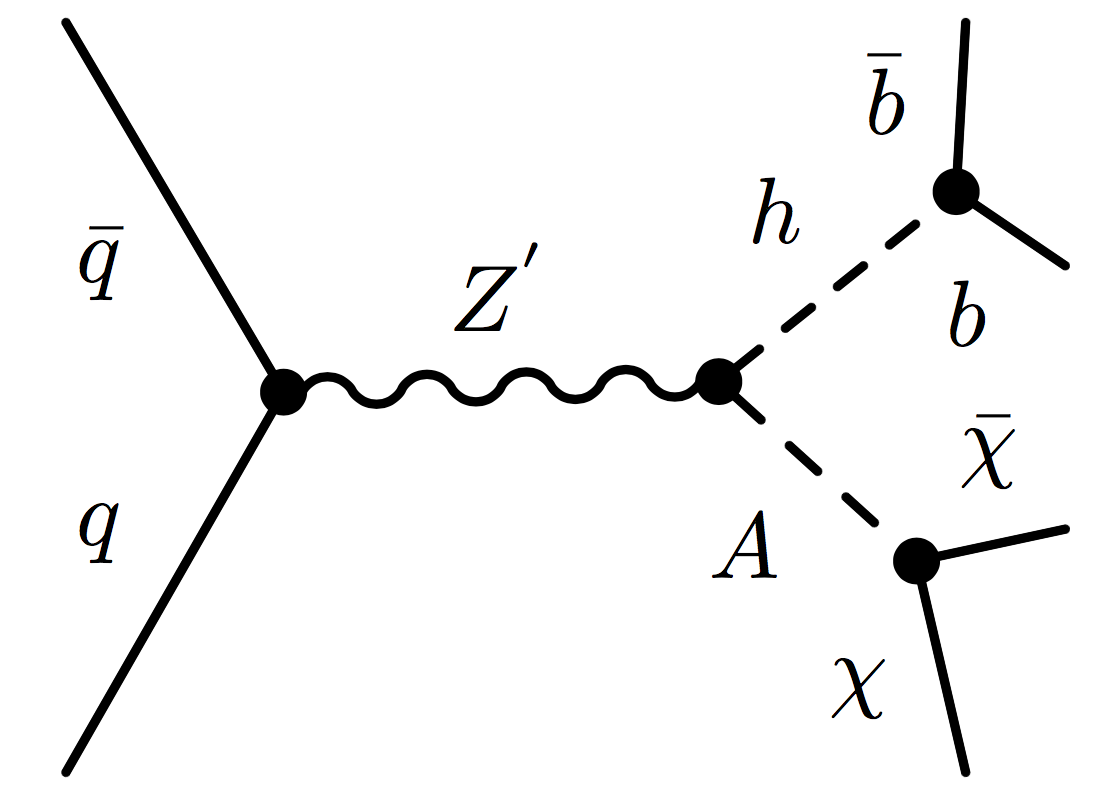
\includegraphics[width=0.8\textwidth]{figures/monohbb}
	\end{minipage}
	\begin{minipage}[b]{0.45\textwidth}
	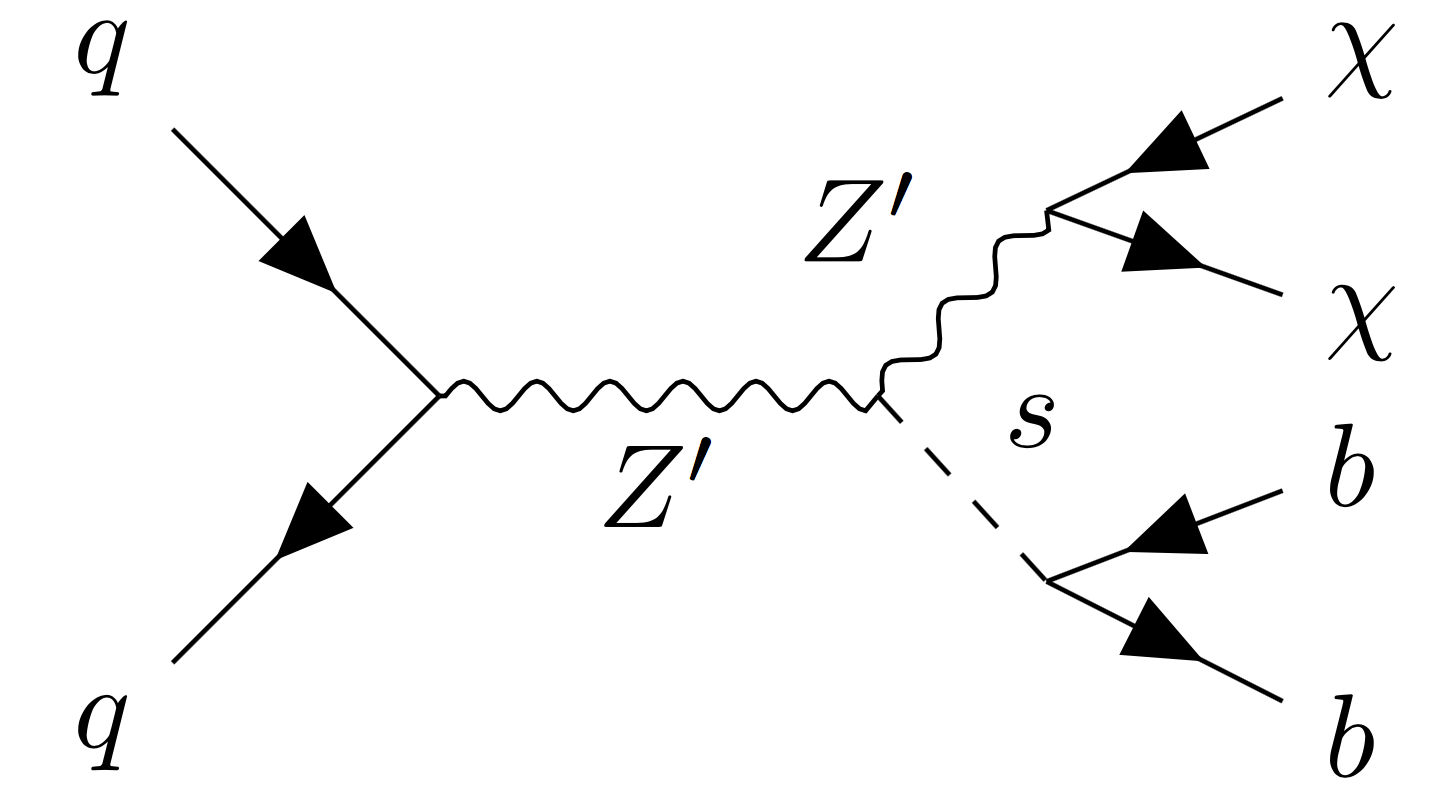
\includegraphics[width=0.9\textwidth]{figures/monosbb}
	\end{minipage}
	\caption[]{Left: Leading-order Feynman diagram representing the model used to interpret the mono-H(bb) dark matter search. Right: A leading-order Feynam diagram representing the model used to guide and interpret the mono-s(bb) re-interpretation of the mono-H(bb) search. The dark higgs mediator mass m$_s$ is allowed to float in the dark higgs model.}
	\label{fig:monohbbreinterp}
\end{figure}

The re-interpreted mono-H(bb) search set limits, shown in figure \ref{fig:monosbb_exclusion}, on the phase space of $Z'$ and $s$ masses excluded by the data. To set these exclusion limits, several free parameters in the dark higgs model need to be fixed. Specifically:

\begin{itemize}
\item The dark matter mass m$_\chi$ is fixed to 200 GeV.
\item The constant g$_q$ associated with the coupling of the $Z'$ boson to quarks is fixed to 0.25.
\item The constant g$_\chi$ associated with the coupling of the $Z'$ boson to dark matter is fixed to 1.0.
\item The mixing angle $\theta$ between the dark and SM higgs bosons is fixed to 0.01.
\end{itemize}

\begin{figure}[H]
	\centering
	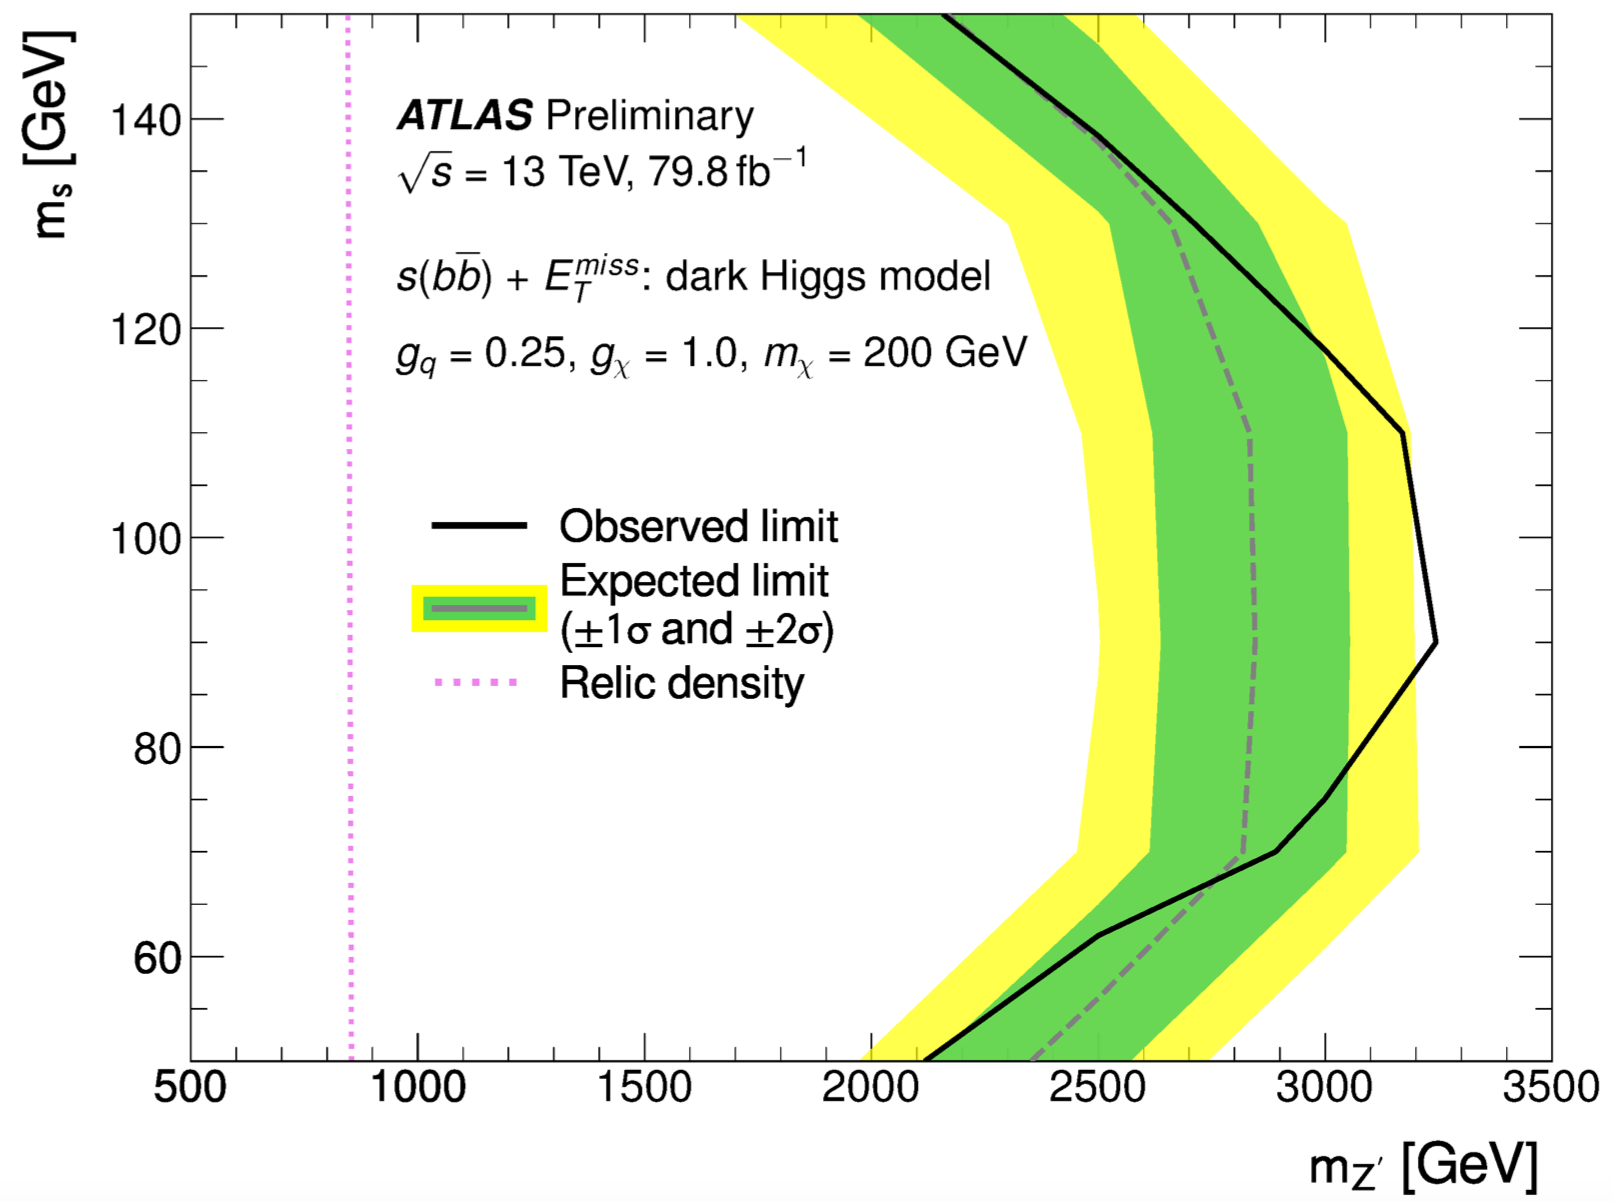
\includegraphics[width=0.7\textwidth]{figures/monosbb_exclusion.png}
	\caption[]{Exclusion limits set on the $Z'$ and $s$ mediator masses by the mono-H(bb) search re-interpreted with the dark higgs model. Mass combinations to the left of the solid black curve are excluded at a 95\% confidence level. Source: \cite{monohbb_recast}}
	\label{fig:monosbb_exclusion}
\end{figure}

The values of $g_q$ and $g_\chi$ were chosen to match the conventional choices used by other LHC DM searches, and $\theta$ matches the choice used in the original paper \cite{dark_higgs} that introduced the dark higgs model.

\subsubsection{Dark Higgs Decay Modes}

The re-interpreted mono-H(bb) search probed the dark higgs model in the case where the $s$ emitted from the $Z'$ mediator decays to a pair of b quarks. However, predictions of the dark higgs branching ratio presented in the re-interpretation paper \cite{monohbb_recast} and shown in figure \ref{fig:higgsbrs} indicate that the $s \rightarrow bb$ decay mode is only sensitive to a range of dark higgs masses up to $\sim$150 GeV, above which the WW decay mode dominates in sensitivity. 

\begin{figure}[H]
	\centering
	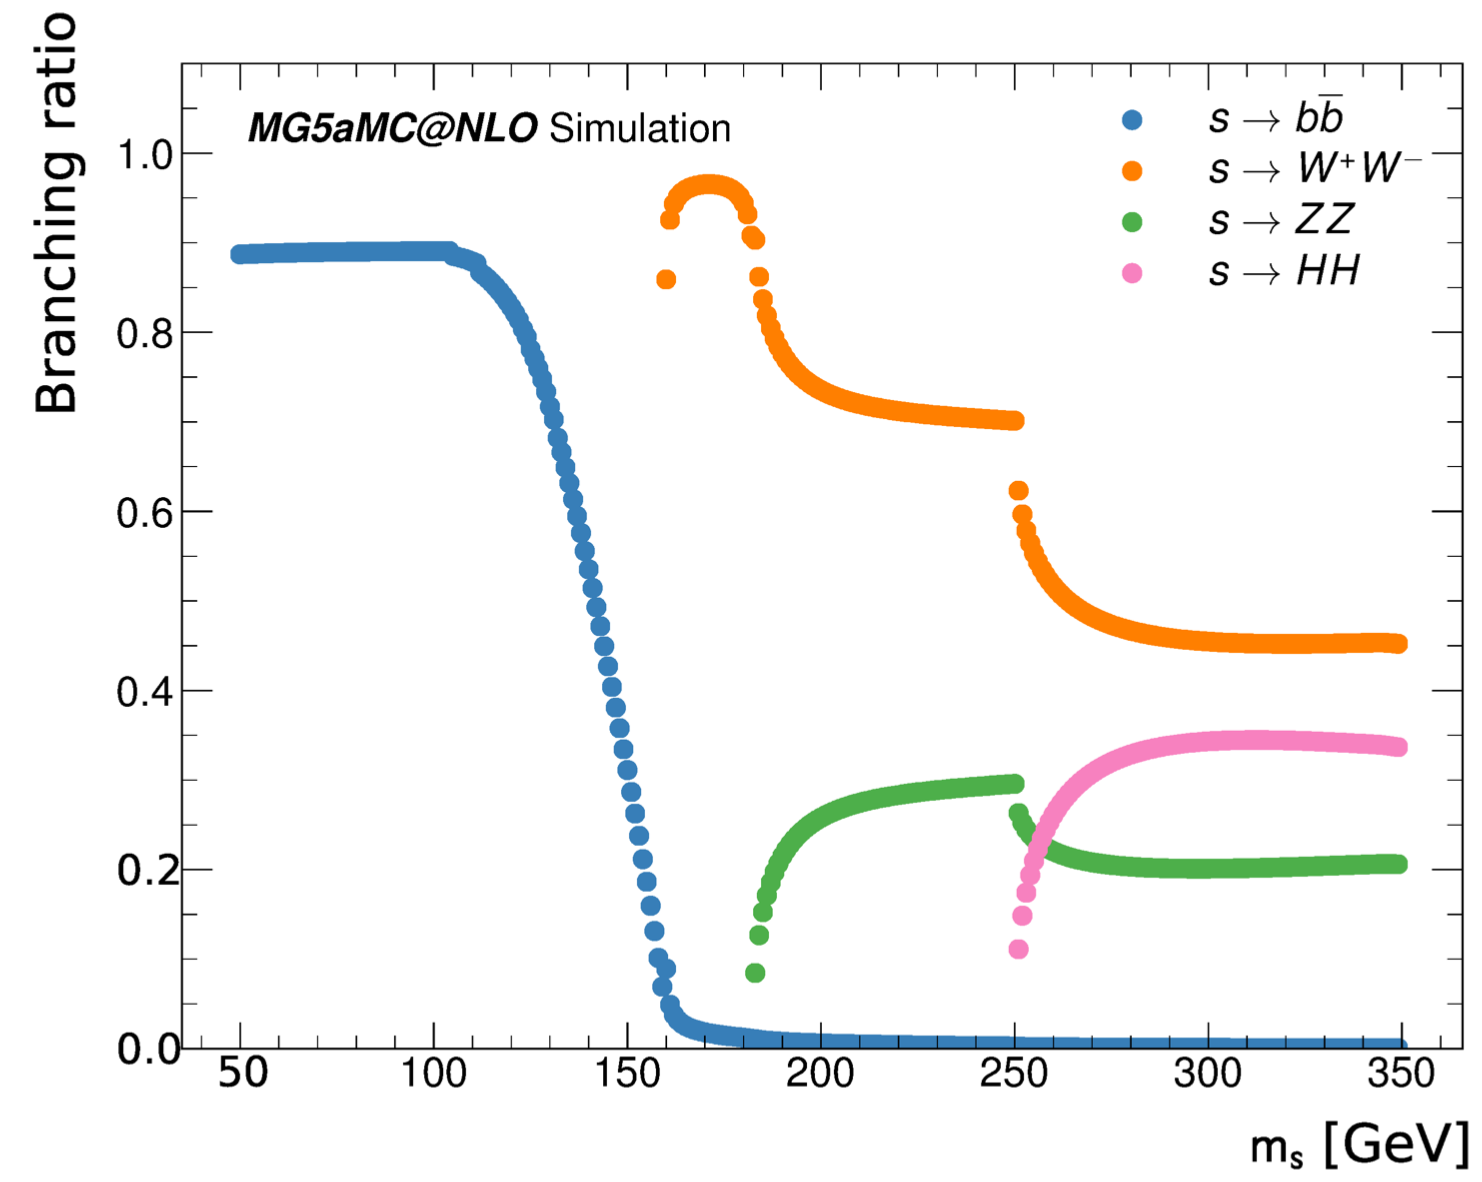
\includegraphics[width=0.7\textwidth]{figures/BR_vs_mass.png}
	\caption[]{Predicted dark higgs decay branching ratios as a function of dark higgs mass. Source: \cite{monohbb_recast} }
	\label{fig:higgsbrs}
\end{figure}

There is no a-priori reason to expect the dark higgs mass m$_s$ to necessarily lie below 150 GeV. Therefore, it's important to probe the model in the higher m$_s$ range by analyzing the $s \rightarrow WW$ decay mode. The proposed thesis work will analyze the latter decay mode using the full 139 fb$^{-1}$ ATLAS run 2 dataset, focusing on the semileptonic final state $WW \rightarrow q\bar{q}\ell\nu$.

\newpage

\section{Introduction to the LHC and the ATLAS detector}

The Large Hadron Collider (LHC) \cite{lhc_machine} is a circular proton-proton collider which resides in a 27 km tunnel near the European Organization for Nuclear Research (CERN). Superconducting magnets are used to accelerate counter-rotating bunched proton beams to high energy, and direct the beams into head-on collisions at four interaction points around the ring. The collisions take place at a world-leading centre of mass energy of up to 13 TeV. 

Each interaction point is surrounded by a detector, which measures the energetic debris of particles produced by the high energy collisions to perform precision measurements of the standard model and search for new physics. ATLAS (A Toroidal LHC ApparatuS) \cite{atlas} is one of two multi-purpose detectors at the LHC, designed to record and study a wide range of physics processes resulting from the collisions. 

The ATLAS detector, shown schematically in figure \ref{fig:detector}, provides full 4$\pi$ coverage around the interaction point, with the exception of the beam pipe. It consists of several layers of sub-detectors, each of which is specialized for recording certain kinematic information and particle types. The sub-detectors are described in some detail below. 

\begin{figure}[H]
	\centering
	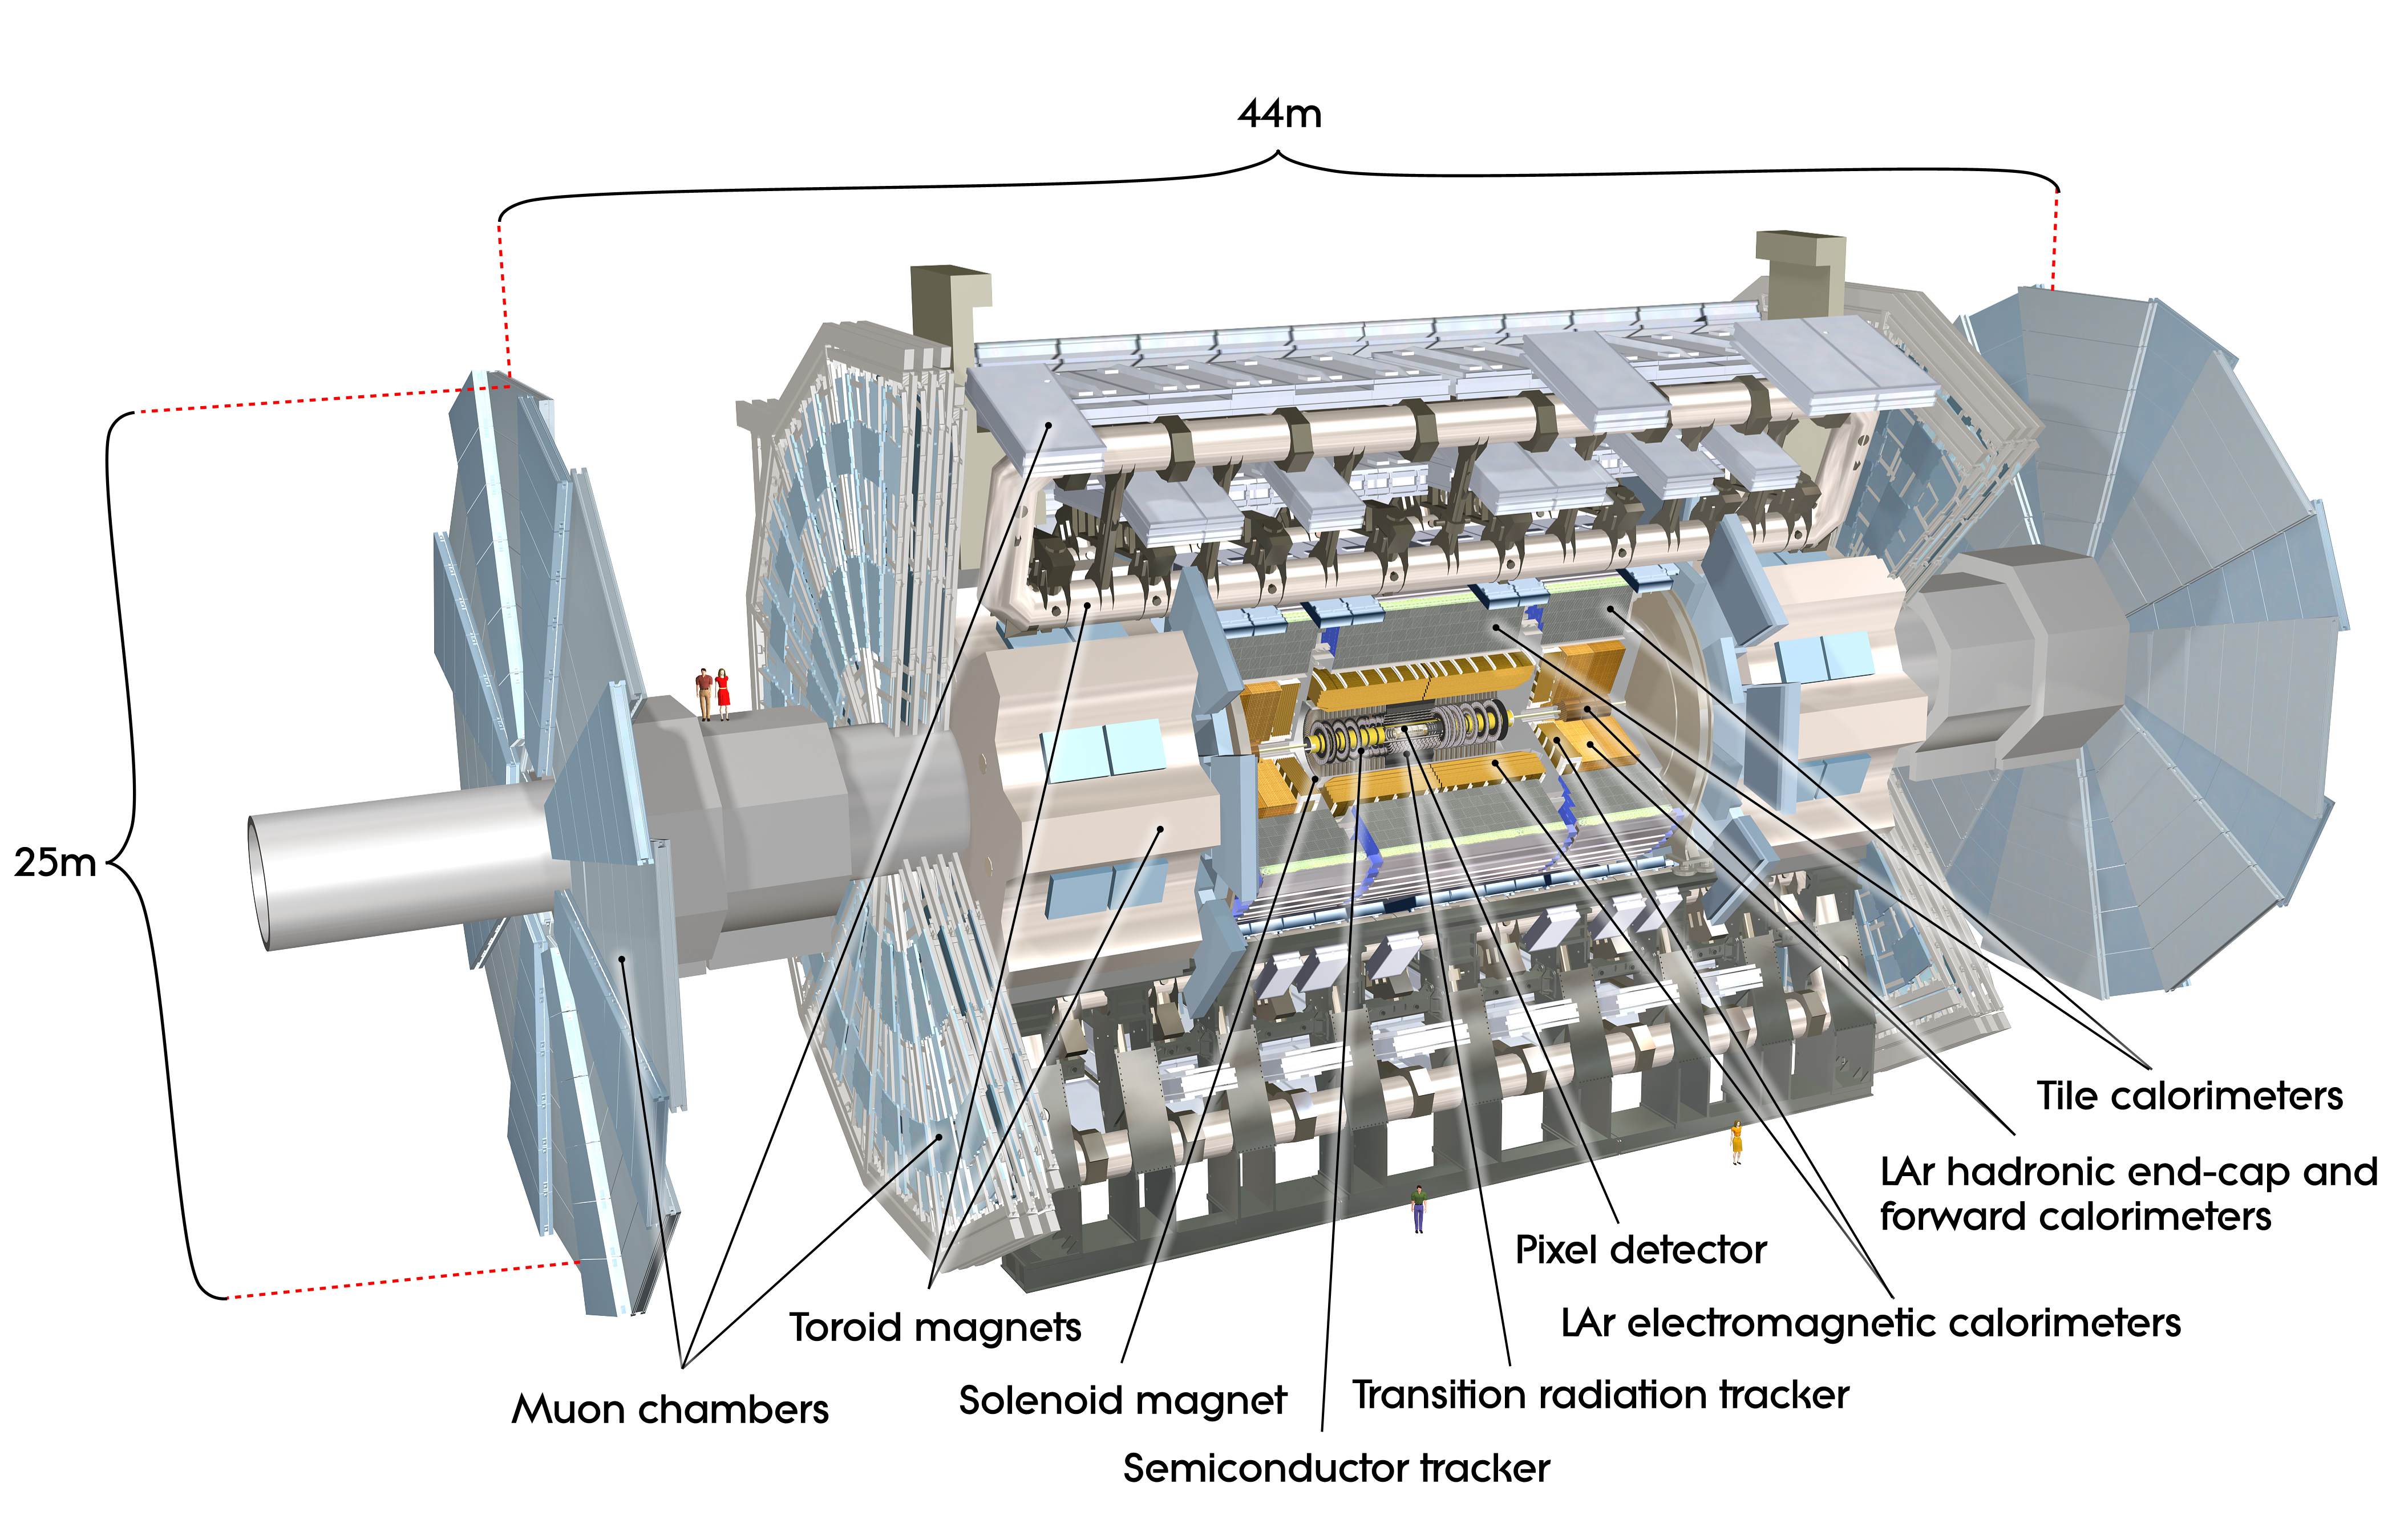
\includegraphics[width=0.85\textwidth]{figures/detector.jpg}
	\caption[]{Schematic diagram of the ATLAS detector. Source: \cite{atlas}}
	\label{fig:detector}
\end{figure}

\subsection{The Inner Detector}

The inner detector (ID), located nearest the the beam pipe, is specialized for charged particle tracking. It is immersed in a 2T magnetic field oriented parallel to the beam pipe, which bends the trajectories of electrically charged particles as they pass through the field. Three distinct but complementary tracking technologies are employed along with pattern recognition tools to map the trajectories of charged particles passing through the ID. These reconstructed tracks are a critical component of vertex reconstruction, and the degree and direction of bent tracks provide information about the momentum, charge, and identity of the charged particles that produced them. 

\subsection{The Calorimeter}

The calorimeter is designed to measure the energy of all particles which pass through it by initiating ``showers" and fully absorbing their energy. The only particles which cannot be absorbed by the calorimeter are muons and neutrinos, which pass through without showering. The calorimeter is divided into two sub-detectors, the electromagnetic and hadronic calorimeters. Both are ``sampling calorimeters", which means they are comprised of repeated layers of dense absorbing material with ``sampling" layers in between. The sampling layers track the location of the shower and record a small fraction of its energy, to which a calibration factor can be applied to infer the full shower energy. 

\subsubsection{Electromagnetic Calorimeter}

The electromagnetic (EM) calorimeter forms the inner calorimeter layer, and is designed to fully absorb and measure the energy of electrons and photons. Energy is deposited in the iron-steel absorbing layers in the form of EM showers \cite{em_showers}, in which the initial electron or photon interacts with the absorbing material to produce a cascade of photon radiation and electron pair production. The sampling layers are filled with liquid argon (LAr), with sensors to measure the ionization produced by charged particles passing through the LAr \cite{em_cal}. 

\subsubsection{Hadronic Calorimeter}

The hadronic calorimeter surrounds the EM calorimeter, and is designed to fully absorb and measure hadronic showers, also known as ``jets", initiated by hadrons, which can make it through the EM calorimeter due to their relatively long interaction length \cite{atlas}. Unlike the EM showers described above which proceed exclusively via electromagnetic interactions, hadronic showers proceed via both the strong and EM interactions, and as a result are in general more variable and less localized. 

The hadronic calorimeter is comprised of a tile calorimeter which encircles the EM calorimeter barrel, and a LAr calorimeter with copper and tungsten absorbers in the end-cap region which encloses the two ends of the barrel. The tile calorimeter uses steel as the absorber material and scintillators read out by photomultiplier tubes (PMTs) in the sampling layers. 

\subsection{The Muon Spectrometer}

The muon spectrometer \cite{atlas} surrounding the calorimeter is specialized for tracking muons and measuring their momentum. It employs the same principle used in the inner detector of applying a strong magnetic field and measuring the resulting bent tracks of the electrically charged muons passing through to infer their momentum. 

The magnetic field is generated by rectangular superconducting ``toroid magnets" arranged radially around the beam axis, which set up a toroidal field concentric to the beam axis. In the region containing the strong field established by the toroid magnets, muon tracks are recorded by three cylindrical layers of muon tracking chambers in the barrel region and three layers of chambers arranged in wheels perpendicular to the beam axis in the end-cap region. Additional layers of fast trigger chambers deliver muon track information to the ATLAS trigger system so it can be incorporated into the event readout decision. 

\newpage

\section{Ongoing analysis of mono-s(WW) hadronic channel}
\begin{itemize}
\item Preselection
\item Signal region selection
\item Control regions
\item Very brief summary of systematics (exp and modeling)
\item Sensitivity estimates
\item RECAST
\end{itemize}

\section{Signal Sample Generation for Semileptonic Channel}

The mass of a dark matter particle is fixed to 200 GeV/c$^2$, and the $Z'$ and dark higgs masses are allowed to vary from 500 GeV/c$^2$ to 2500 GeV/c$^2$ and 160 GeV/c$^2$ to 360 GeV/c$^2$, respectively. 

\begin{figure}[H]
	\centering
	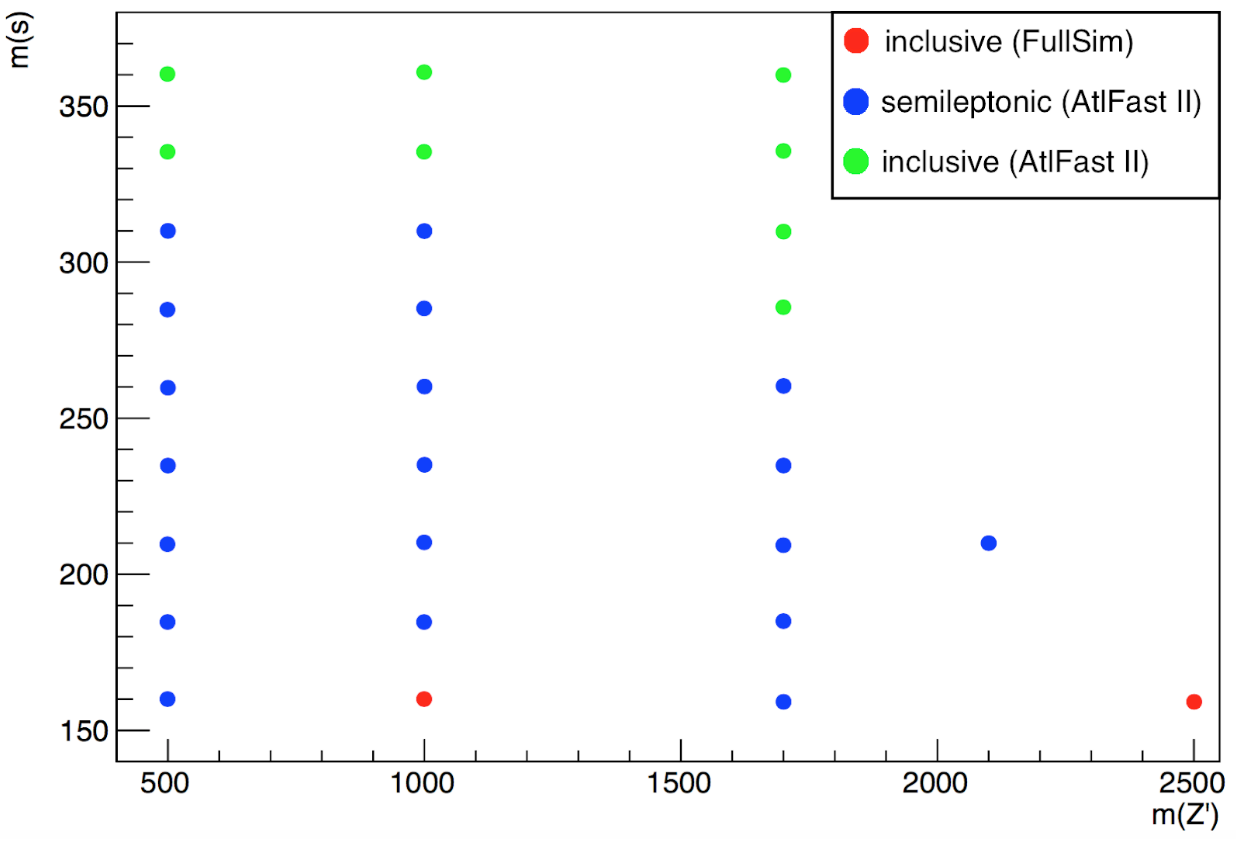
\includegraphics[width=0.7\textwidth]{figures/SignalGrid.png}
	\caption[]{Grid of signal points with respect to dark higgs (s) and $Z'$ boson masses of generated signal sample}
	\label{fig:signalgrid}
\end{figure}

\begin{itemize}
	\item Scan over range of m($s$) and m($Z'$)
	\item Need to fix some parameters in the model:
	\begin{itemize}
		\item $g_{q} = 0.25$
		\item $g_{\chi} = 1$
		\item $\theta = 0.01$
		\item $m_{\chi} = 200$ GeV
	\end{itemize}
	\item Discuss motivation for above choices of fixed model parameters
\end{itemize}

\section{Event Selection for Semileptonic Channel}

\subsection{Preselection}
\begin{itemize}
\item MET trigger passed
\item 1 signal lepton
\item MET > 150 GeV
\end{itemize}
\subsection{Regions}
\begin{itemize}
\item Signal region
\item W+jets control region
\item ttbar control region (if we plan to do one)
\end{itemize}
\subsection{Categories}
\begin{figure}[H]
     \centering
     \begin{subfigure}[b]{0.4\textwidth}
         \centering
         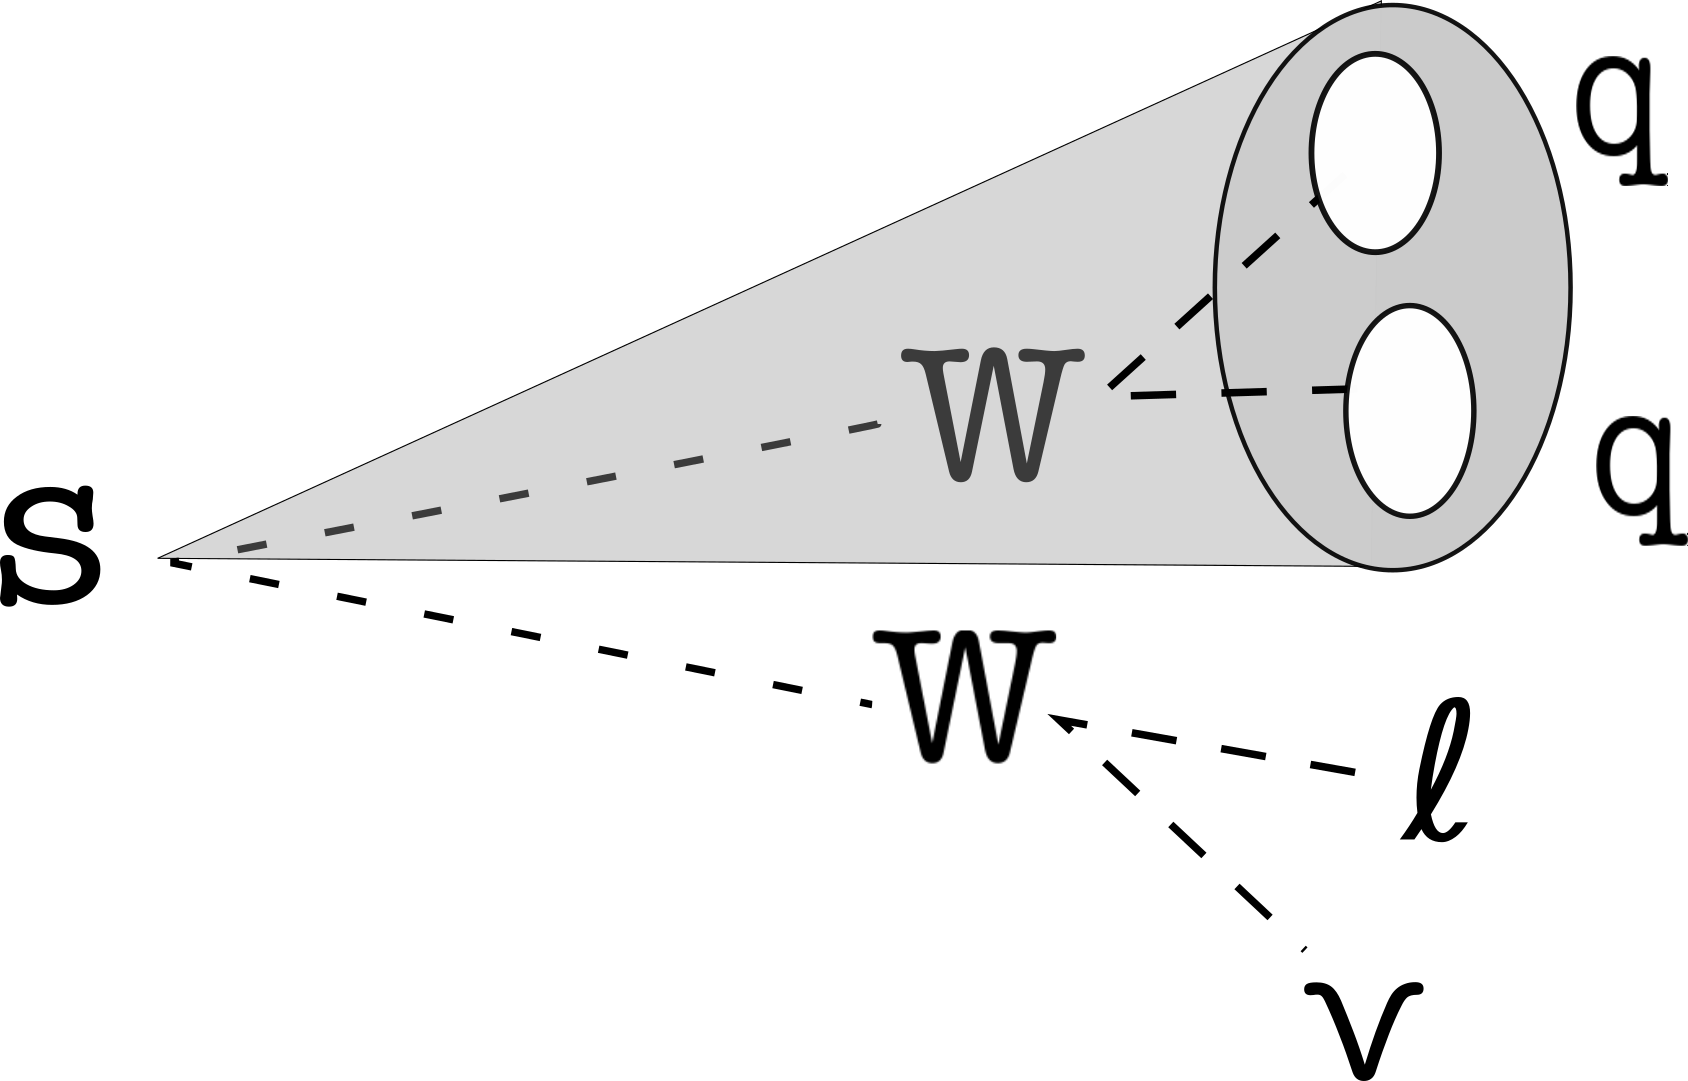
\includegraphics[width=0.9\textwidth]{figures/merged.png}
         \caption[]{Merged category}
         \label{fig:merged}
     \end{subfigure}
     \hfill
     \begin{subfigure}[b]{0.4\textwidth}
         \centering
         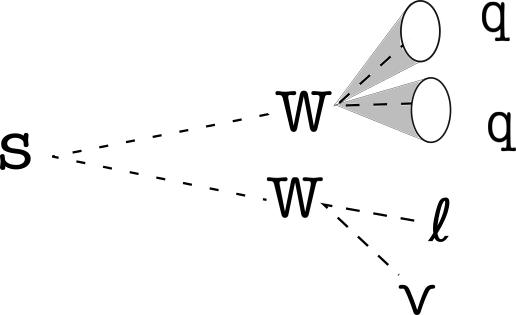
\includegraphics[width=0.9\textwidth]{figures/resolved.png}
         \caption[]{Resolved category}
         \label{fig:resolved}
     \end{subfigure}
\caption[]{Kinematic categories for final state selection}
\label{fig:categories}
\end{figure}
\begin{itemize}
\item Resolved category
\item Merged category
\end{itemize}


\section{Sensitivity Studies}
\subsection{Background on limit setting}
\subsection{HistFitter setup}
\begin{itemize}
\item Fit variable
\item Binning
\item Use of temporary systematics proxy
\end{itemize}
\subsection{Preliminary sensitivity limits}
\begin{itemize}
\item Resolved 
\item Merged 
\item Combined
\end{itemize}

\section{Remaining Work and Outlook}
\begin{itemize}
\item Study variables to help address $p_\nu$ vs. $p_{\chi\bar{\chi}}$ MET ambiguity
\item Finalize SR and CR definitions
\item Experimental and modeling systematics
\item Finalize sensitivity estimates with final systematics
\item Statistical combination with hadronic channel for combined limits
\end{itemize}

\newpage

\bibliography{bibliography}
\bibliographystyle{unsrt}

\end{document}